\chapter{HTML Page Layout Using CSS}
\label{layout}
\paragraph{} HTML alone is really great, but pretty ugly. CSS gives us a way to improve how our pages are presented. We can use CSS and semantic HTML to group and organise elements of the UI to give us reusable ``blocks'' or `units'' from which any given page is assembled.
\paragraph{} The last chapter only scratched the surface of CSS and its interaction with, and applications to, Web design. We'll continue our study of CSS, but this time with a focus on the specific ways that CSS supports ``laying out'' or arranging the elements of a web page to achieve a particular design. You should contrast this with the last unit where we considered how individual typographical elements could be styled, such as the size or colour of lines of text. 
\paragraph{} Now, instead, we're thinking a little bigger, how all of the elements of a page work together to implement a design. Part of this story will be continued in the next unit when we consider some rules of thumb for designing pleasing user experiences. 
\paragraph{} For now though we'll consider how any given page can often be considered in terms of a number of blocks. Each block will gather together a number of html elements, for example, the header block, the footer block, the main content or "body" block, and the navigational block. When we start to think of our pages in terms of reusable blocks it can assist us both in designing our pages but also in terms of  implementing them as well.
\paragraph{} We've seen how HTML gives us essential structure for turning plain text documents into hypertext documents. To some degree HTML also gives us many of the structural elements that we are already used to in terms of word processing text documents. When we decide to make a line into a heading or add a break in our text to create a paragraph, these are similar processes whether we are using a word processor or writing HTML. However, these choices are concerned with capturing, or delineating, the different ways in which the parts of the document work together. Just marking something as a heading or a paragraph doesn't necessarily mean that it must be presented in any specific way. Instead it marks it out so that we can, if so desired, present it in a different way. This marking up process merely facilitates our being able to achieve this.
\paragraph{} To actually make a difference to how our HTML document, and the elements that make up that document, are actually seen by a user, we need to consider presentation. We use CSS to govern the visual presentation of our document, using the various elements of our HTML markup as cues to help us achieve this. 
\paragraph{} However, whilst CSS is concerned with visual presentation, this is not just making things look pretty. In addition, visual presentation via CSS is an important aspect of both usability and accessibility. By usability we mean all aspects of the design that make the resulting rendered page fit to address the task for which it was intended. Usability can range over many factors including safety, effectiveness, and efficiency. Accessibility is a related topic to usability which is concerned more with ensuring that the resulting design doesn't exclude users from effectively using it. This could include ensuring that a page is accessible to people with specific disabilities, for example, making a page accessible to those with visual impairment might require the underlying HTML to be effectively structured for an assistive technology such as a screen reader to use it. However not all visual impairments are equal, another view on the same aspect of accessibility might require that colour contrast be sufficient between background and foreground elements so that those with minor visual impairments can effectively use the site, whereas colour selection, the choice of colours for a site's colour scheme shouldn't exclude those, or reduce accessibility for those with colour vision deficiency or colour blindness. To root this in the real world consider that red-green colour blindness affects up to 8\% of males of Northern European descent.
\paragraph{} In the last unit we dealt with styling individual elements but now let's consider how we can group HTML elements together so that they can be managed, laid out, and presented to our users regardless of the device they use. By doing this kind of approach, we also start to gain some strategies for managing a site's design, rather than merely the design of a single page. By reusing groups of elements in similar ways across different pages, we can begin to produce designs that have consistency, and which, as a result, provide a better user experience.
\paragraph{} Before we get deeper into this unit, let's also consider just how good the browser is at rendering web pages. Whilst CSS is useful for styling HTML and can make things look great, allowing the browser (user agent) to decide how to place HTML elements on screen is frequently a great idea. The main reason is that this is what the browser, or more correctly, the browser's page layout engine, is designed to do. You can however override this behaviour to get your pages to be laid out and rendered in other ways. CSS will influence how things look and where they are placed. You should recognise though that the more you override the browsers default approach to page layout, the more work you are making for yourself and the more likely you are to run into cross-browser inconsistencies that can lead to different behaviour on different platforms.


\section{Rendering Pages}
\paragraph{} Our browser is designed to render web pages. That is, it retrieves the HTML for the page associated with the current web address, then retrieves any linked resources including CSS and JS as well as things like images. During this process the browser will parse the HTML and create an internal DOM representation of the page, modifying this as necessary to account for any directives from the CSS or any modifications imposed by the JS. 
\paragraph{} Unless the CSS or JS overrides the default layout that the browser uses then most pages are laid out fairly simply. Assuming a left-to-right reading order, rendering begins at the top left corner and the page flows from there in the order in which it is defined in the HTML document. This is generally a straightforward process which, as a rule, is only hindered by images of unknown dimensions which take longer to download than the rendering engine takes to layout the page according to the known information. This is one reason why you might occasionally see pages that seem to change where things are located as images appear, because the dimensions weren't specified in the HTML and could only be finalised once the associated image file was fully retrieved.
\paragraph{} Sometimes though, we really want to have more control over our layout. We want to be able to create a block, or grouping of items, that are placed in a specific location on screen, e.g. to the left, or right, or above, or below other items. Essentially we want to place our HTML elements in particular locations on screen where the normal layout engine, uninterrupted, wouldn't normally put them. This creates tension because browsers are built around layout engines which are optimised for presenting documents, particularly documents that have a quasi-academic publication style structure including, for example, an introduction, various sub-sections, and a conclusion.
\paragraph{} Any other form of screen layout, such as a desktop application style user interface, will potentially cause issues for the layout engine. For example, requiring multiple passes to place things in their correct position, or even not being able to consistently and comprehensively satisfy all of the constraints that the design imposes. Remember also that the rendering engine is trying to, by default, create the best layout for the current combination of screen quality and window dimensions, given the content that has to be displayed, and, for the most part, the current generation of rendering engines do a really good job when designers respect this.
\paragraph{} We should note that text is inherently responsive by default. It can keep wrapping to the next line until you reach the end of the content. Text resizes nicely to account for all devices, screens, viewports, and window sizes, resolutions, pixel densities, and dimensions. It just keeps flowing until the page is done. 
However when we try to use the same rendering engine for more exacting layouts, trying to implement desktop style interfaces for example, difficulties can, and frequently do, arise.



\section{Layouts: HTML + CSS}
\paragraph{} Let's now look at a way to do layouts with CSS and HTML versions earlier that HTML5 that you will see in the wild, and which work, but that are no longer the preferred approaches. Note that this is for historical usage only; we'll look at some better ways to implement modern designs using HTML5 and CSS, but currently you also need to be aware of the approaches that are still out there. Because many sites have used these approaches, they will be around for a long time, and you might be called upon to maintain such a site in your career.
\paragraph{} You can use HTML <span> and <div> elements to assemble page layouts. These elements work in different ways and introduce two useful notions to our design toolset. The first is the idea of an inline element, something that works within the context of, or inline with, another element. For example, given a paragraph of text, if you want to have a specific sub-string treated in a different way, such as coloured for emphasis, then an inline element is useful to mark up the start and end of the sub string. The span element is just such an inline element and that's exactly how we might use it. Contrast that with the div element which enables us to wrap parts of our page into a block, to group elements, so that we can treat the contents of the block differently from the rest of the page.
\paragraph{} If we wrap these inline and block elements around the different groups of content of our page we can then target those groups with specific CSS. This is achieved by given each inline and block element a unique ID attribute so that they can be identified, referenced, and subsequently positioned and styled by CSS. Note that to do this, HTML requires IDs to be unique.
\paragraph{} You'll see this pattern in lots of web sites built prior to HTML5. For quite a while this was an effective way to control the layout of a page but it had, and still has, drawbacks. The main drawback is that your choice of ID for each grouping might not have the same semantic communicative ability as the IDs that others are using. Also the sheer variety of ways in which we can say the same thing, e.g. referring to the navigation bar which we could call ``navigation bar'' or just ``navigation'' or ``navbar'' or ``nav-bar'' or merely ``nav''. If it is a panel down the side then we can add all the combinations of nav and panel to the list above. Instead it is best to use semantic HTML tags to achieve this kind of layout control when possible. 
\paragraph{} But what if you have groupings that don’t fit to standard semantic tags? For example, for columns of content in a multi-column layout for ultra-wide monitors. At this point, the use of div blocks makes sense again, as a way to take us beyond the language that HTML 5 semantics define, but not as a starting place.


\section{How Not To Lay Out Pages}
\paragraph{} Using div and span tags to organise a page layout isn't the only way that web developers have tried to produce pixel perfect layouts and desktop style user interfaces in the past. So let's quickly survey some of the approaches for how not to do it.
\paragraph{} One method was to misuse HTML tables. Because tables arrange things semantically into columns and rows, it is an easy mis-step to get from there to the idea that this semantic use can extend to the visual presentational use. However tables are, just like most default HTML elements, inherently responsive, they will reflow to best fit the screen and window that they are rendering for. This means that changing the window dimensions can alter the layout of the page contents as the text reflows. A clever hack involved combining a table with single pixel transparent gif image files. As they are transparent, the user doesn't see the files, but by using many of them they can be used to push page content around so that it is laid out just as the designer intended for it to be seen visually. However, this is a horrible solution to the problem of getting HTML layout engines to do something they weren’t designed to. The main problem being that this is not easily maintainable and can have lots of side-effects for accessibility because a page might now incorporate many thousands of instances of transparent gifs. Think about it, to indent a line of text by 300 pixels will need 300 single pixel gifs.
\paragraph{} In comparison to this, the use of divs and spans to group elements then CSS to arrange them is much better; whilst this is still horrible and severely breaks semantic HTML the impact is less terrible but far from ideal.



\section{Some Common Layouts}
\paragraph{} Before we get to actually using CSS to lay out our pages, let's just consider some basic layouts that are quite common.
\paragraph{} The default for the web is as a single column of text which reflows according to the dimensions of the window that it is rendered to. This is inherently reliable, stable, and responsive. However, as the size of page content increases, this can become a little unwieldy, not necessarily unusable, but, for example, the amount of scrolling required to reach the top or bottom of the page can increase significantly. Similarly, such a page might require the user to find the exact hyperlink, embedded in the page, to enable them to navigate to other pages in the site.
\paragraph{} This leads to the category of layouts that involve two parts, the content part, and the navigational part. By grouping all of the links to other pages in the site together, a consistent navigation experience can be designed and replicated relatively easily across all pages in the site so that your users know where to look to find the next place to navigate to. This is generally laid out in one of four ways, with navigation above, or below, or to the left of, or to the right of, the page content. Frequently this leads to a two column layout, with a navigation bar to the left, or right, and the content next to it. This might also include CSS directives to stop the navigation element from scrolling when the rest of the content is bigger than the screen.
\paragraph{} Yet another, reasonably common layout, again with multiple possible variations is the three column layout, including a navigation bar and content, but now with the addition of some kind of sidebar which perhaps incorporates additional data or metadata about the current page.
\paragraph{} You are only really limited by practicality in terms of potential layouts involving some combinations of multiple rows or columns. Note however that a common extension of these layouts is also to include a header and, or, footer area at the top and, or, bottom of the screen respectively. These might well also combine with the navigational aspects, depending upon your design goals for the page.
\paragraph{} Additionally, consider that many sites will also incorporate some dynamic elements in their page layout, for example, enabling hide-able panels or modals that can be shown or hidden as necessary.



\section{CSS-based Layout Solutions}
\paragraph{} Two recent solutions give better control over relative placement of HTML elements than using divs and spans and can enable us to realise some of the layouts we've considered whilst maintaining much of the basic flexibility and responsiveness of traditional HTML. These include the FlexBox and the Grid layout. Each is potentially applied to multiple collections of elements to place them relative to each other on screen during rendering.
\paragraph{} The Flexbox is a way to lay out linear collections of elements either horizontally or vertically. That basically means placing collections next to each other, from the left edge of the screen until the right edge is met, then wrapping around to put the next collection below the others and continuing to place collections in this manner, wrapping around as needed, until everything is laid out. If we consider each collection to be a word in a sentence, which is really a collection of letters, then this is just like how a sentence is placed on a page, running from left margin to right, and wrapping around into another line each time it reaches the right margin.
\paragraph{} The Grid Layout is similar, but instead of working in a single, linear dimension, it works in two dimensions, and is a way to lay out matrices of elements as rows and columns. In some ways this is just a like a table, but recall that an HTML table is for organising matrices of information semantically, a Grid layout is for presenting matrices of information visually. This means that if we want to enforce that a certain group of information is always vertically aligned above or below another group, or immediately to the left or right of another group, we now have a mechanism to do so.
\paragraph{} Both the Flexbox and Grid are designed to use CSS to influence the visual placement of HTML elements so that we can avoid hacks like using the transparent gif when attempting to implement our desired layouts.
\paragraph{} When considering the use of FlexBox and Grid layout we should take into account the following:

\begin{itemize}
\item How we build interfaces — there are certain recurrent patterns of user interface layout as we considered earlier.
\item How pages are rendered — from the upper left corner of the screen to the lower right corner of the screen.
\item That the screen has two dimensions — the horizontal dimension and the vertical dimension.
\end{itemize}

\paragraph{} So, in some cases we want to lay out things in one single dimension, either horizontally or vertically, but not both at the same time. This leads naturally to the idea of the FlexBox. A layout for a collection of items along a single dimension. Where the FlexBox works either horizontally or vertically, if we add the second, complementary, dimension, then we arrive at the Grid layout.
\paragraph{} Let's now consider each approach in turn, starting with the FlexBox\dots



\section{FlexBox}
\paragraph{} Imagine a box reaching horizontally from one side of the screen to the other. This box can contain HTML elements, either as individuals, or in groups. We want to be able to control how elements are spread across the box from one side of the screen to the other. For example, we might want to control the amount of space to either side of, and between, the elements in the box.
\paragraph{} Because our computer screens are not infinitely wide or high, we can't have our box containing infinite elements. At some point, if we have sufficient content, we reach the edge of the screen, and the responsive nature of our browsers rendering engine will attempt to reflow the content to start on the next "line" below. If our screen is too narrow for the content we want to display then we might also want to be able to exercise a little control over how and when the box flows over into another row and arranges elements below.
\paragraph{} Note that there are some minor differences between horizontal and vertical arrangements because we are habitually used to scrolling up and down a page, but less used to scrolling horizontally, so reflowing content that is too wide for the screen so that it is displayed below seems sensible, but for vertical arrangements, we expect to just keep scrolling down until we reach the end.
\paragraph{} Flexbox lets us do this. It supports a range of CSS properties:

\begin{itemize}
\item flex
\item flex-basis
\item flex-direction
\item flex-flow
\item flex-grow
\item flex-shrink
\item flex-wrap
\end{itemize}

\paragraph{} For each property you should investigate the documentation associated with it in the Mozilla developer Network CSS reference\footnote{\url{https://developer.mozilla.org/en-US/docs/Web/CSS/Reference}}. Let's now consider some examples to see what FlexBox looks like and how it can be used.




\section{Flexbox Resizing Example}
\paragraph{} This example is meant to demonstrate a very simple collection of content and how FlexBox can manage the arrangement of that content when a window's dimensions are altered. We'll use FlexBox to style an unordered HTML list.
\paragraph{} First, some HTML (flex1.html) for our page. It's worth taking a look at how this is rendered without the CSS so that you get an idea of what it looks like in isolation without any CSS applied. This will let you see just how much functionality the CSS Flexbox declaration adds.

\begin{lstlisting}
<!DOCTYPE html>
<html lang="en">
	<head>
		<meta charset="UTF-8">
  		<title>CSS Flexbox</title>
  		<link rel="stylesheet" href="flex1.css">
	</head>
	<body>
		<ul class="flex-container">
			<li class="flex-item">1</li>
			<li class="flex-item">2</li>
			<li class="flex-item">3</li>
			<li class="flex-item">4</li>
			<li class="flex-item">5</li>
			<li class="flex-item">6</li>
		</ul>
	</body>
</html>
\end{lstlisting}

\paragraph{} Note that we just have a simple HTML document, with a link to an external CSS file. In the body of our document we merely have an unordered list whose contents are the numbers 1 through 6. This is merely to make it easy to see and compare how the contents of the FlexBox are placed and rendered. See that the <ul> tag has a flex-container class attribute and the individual items are given flex-item class attributes. Now let's get to the CSS (flex1.css).

\begin{lstlisting}

.flex-container {
  padding: 0;
  margin: 0;
  list-style: none;
  display: flex;
  flex-flow: row wrap;
  justify-content: space-around;
}

.flex-item {
  background: tomato;
  padding: 5px;
  width: 200px;
  height: 150px;
  margin-top: 10px;
  
  line-height: 150px;
  color: white;
  font-weight: bold;
  font-size: 3em;
  text-align: center;
}
\end{lstlisting}

\paragraph{} All we have done here is apply styling to the unordered list container, indicating that we want it treated as a flex container with the display:flex and flex:flow directives. We've also applied a style for individual items within the container. This is all standard CSS and not specific to the FlexBox container but merely changes colour and font settings, as well as adding padding and sizing information to the elements.
\paragraph{} This should give us a set of 6 boxes which will reorganise themselves to best use the space available in the enclosing window. Here is what it should look like but you should really try it out for yourself and experiment with things to get a feel for how the FlexBox acts.


\begin{figure}[H]
\centering
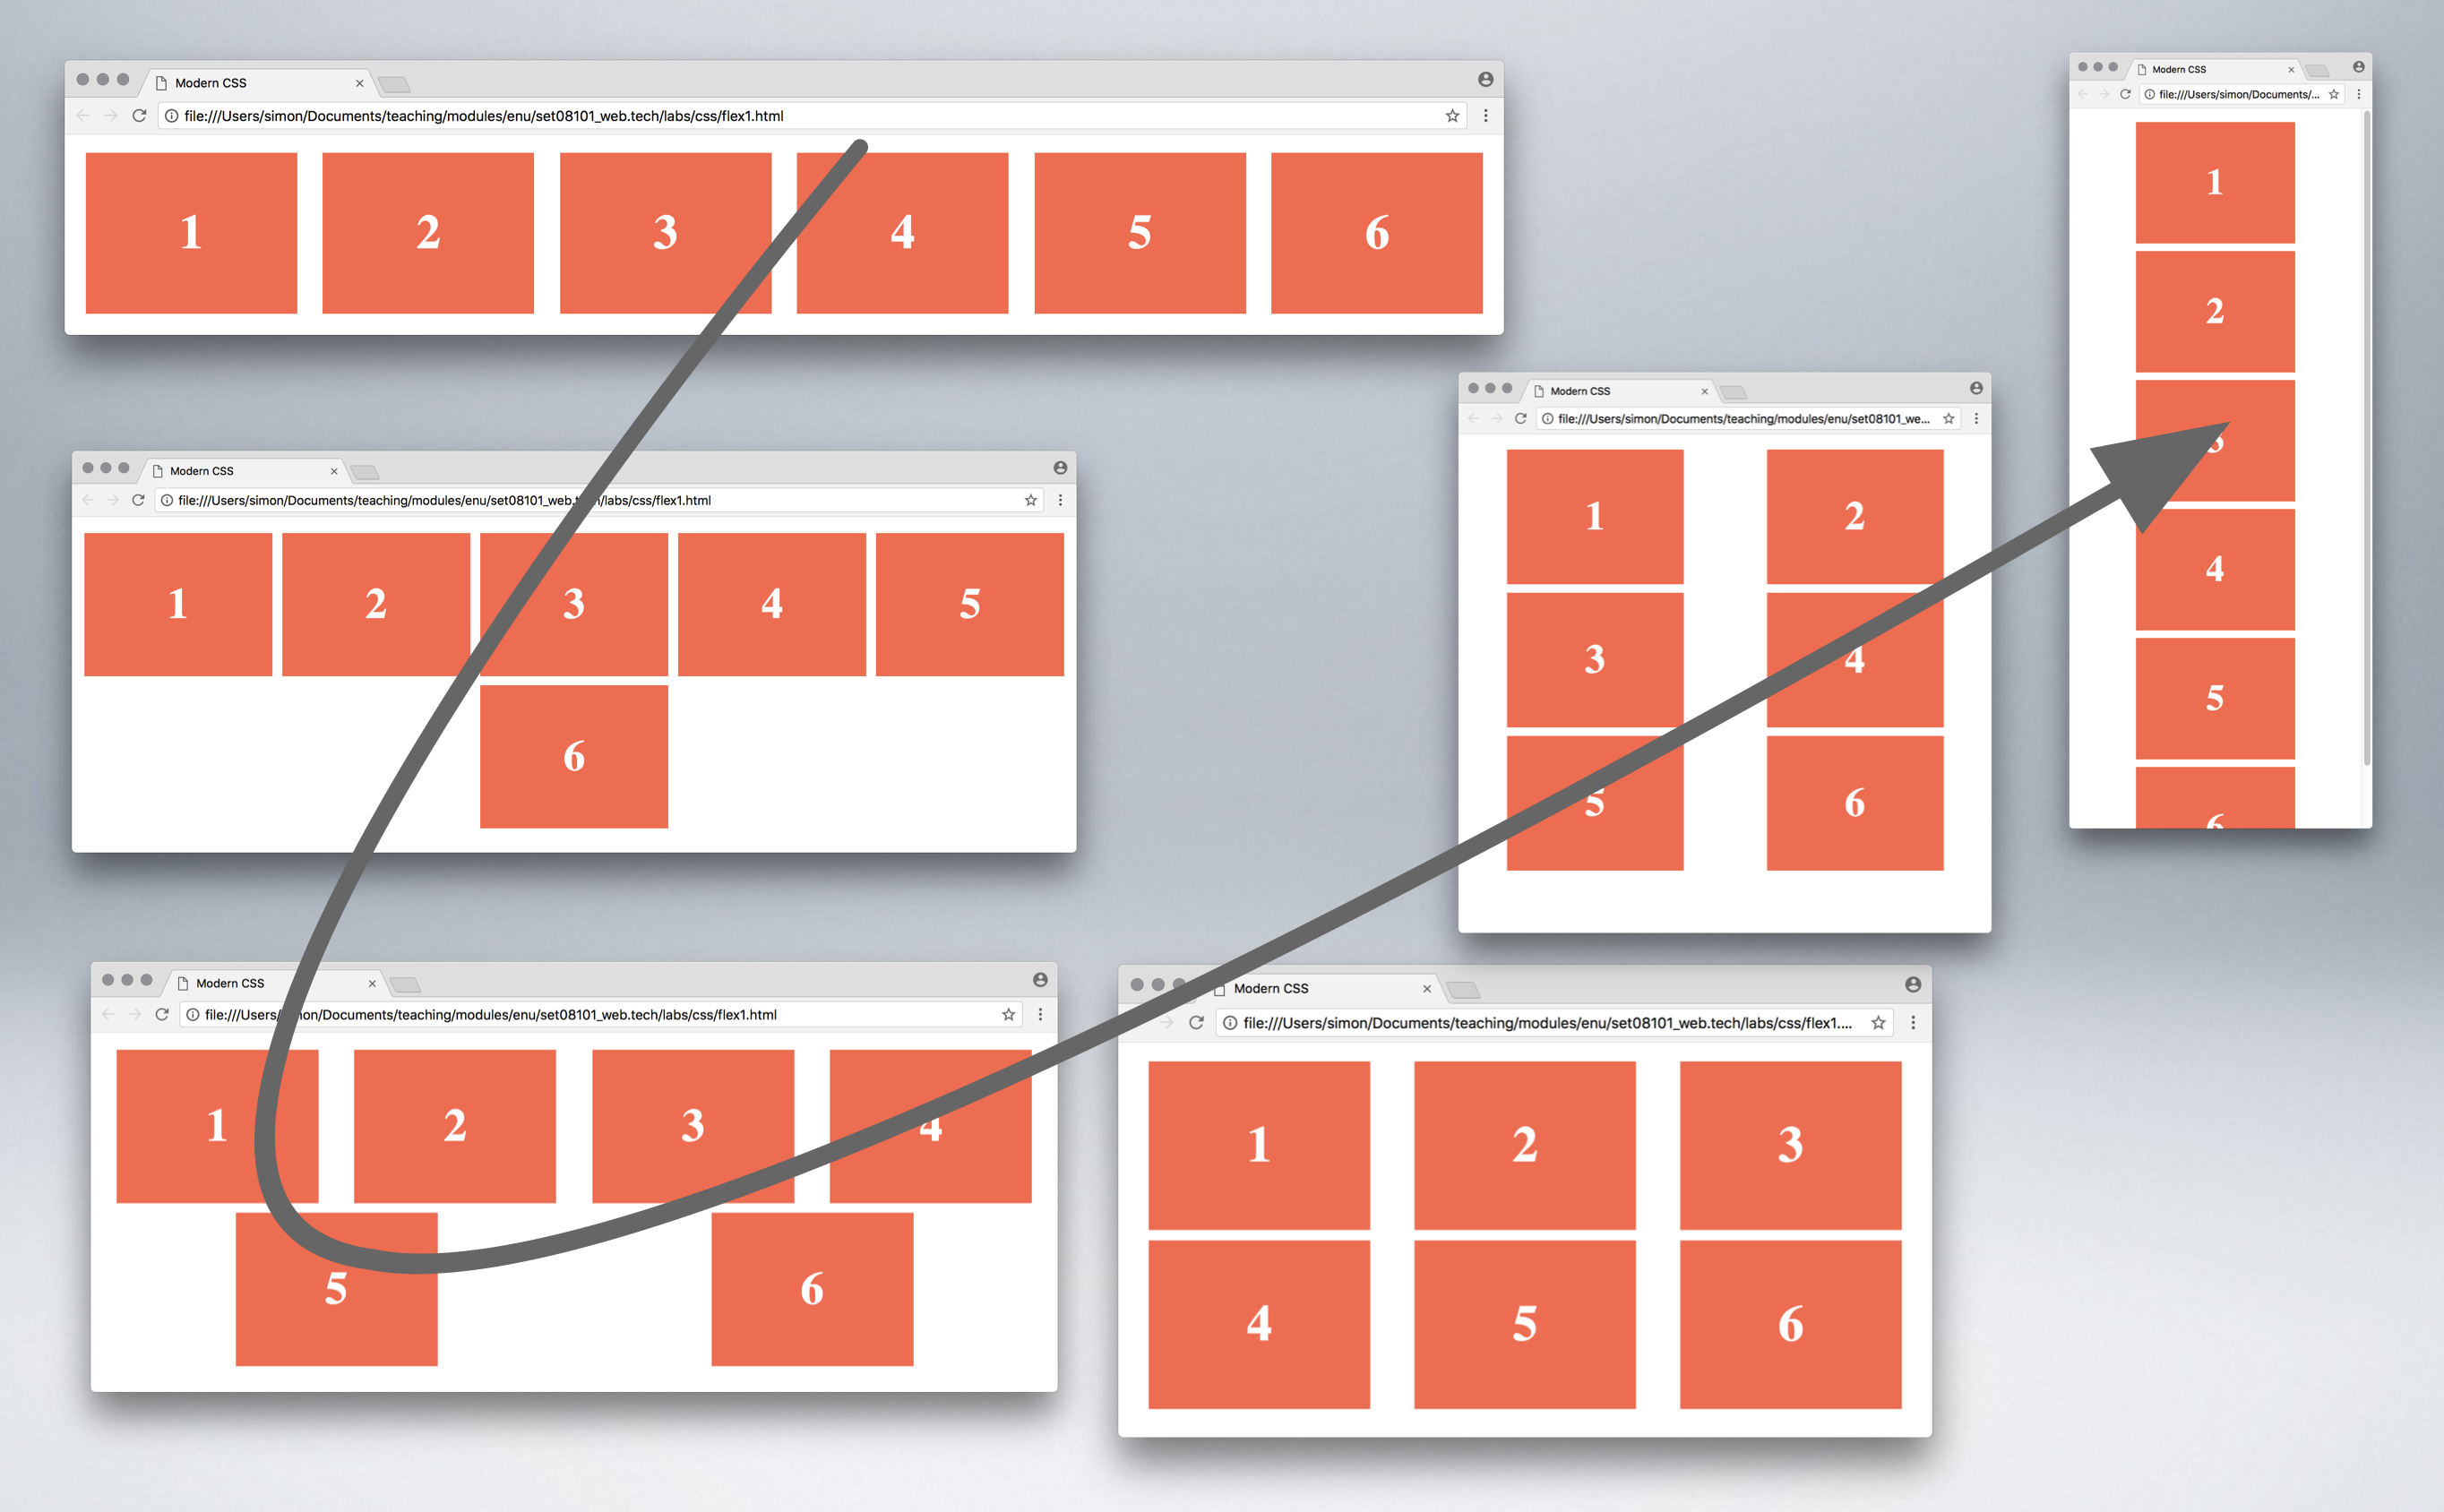
\includegraphics[width=0.8\textwidth]{figures/flexbox-resizing-example}
\label{fig:flexbox-resizing-example}
\caption{}
\end{figure}




\section{Flexbox Navbar}
\paragraph{} One useful application of the FlexBox is to help implement a navigation bar, or navbar, which will reflow to make the best use of the enclosing window whilst remaining enclosed and isolated from surrounding HTML elements in the same document. This is a common layout design that is worth having in your toolbox.
\paragraph{} Let's see what a simple navbar would look like using the FlexBox. First some HTML (flex2.html):

\begin{lstlisting}
<!DOCTYPE html>
<html lang="en">
	<head>
		<meta charset="UTF-8">
  		<title>Flexbox Navbar</title>
  		<link rel="stylesheet" href="flex2.css">
	</head>
	<body>
		<ul class="navigation">
  			<li><a href="#">Home</a></li>
  			<li><a href="#">About</a></li>
  			<li><a href="#">Products</a></li>
  			<li><a href="#">Contact</a></li>
		</ul>
	</body>
</html>
\end{lstlisting}

\paragraph{} This is fairly straightforward HTML content. Like our last example, an unordered HTML list, but instead of merely numbers as content, we've named each item according to how it might be named for a simple online business, and turned each item into an empty hyperlink because the purpose of a navbar is to help us to navigate to different locations in the site. Now let's investigate the CSS (flex2.css) to style this as a FlexBox navbar. It's a bit more complicated than the simple demonstration earlier. If in doubt look up the CSS declarations that you are unfamiliar with in the MDN CSS reference.



\begin{lstlisting}
.navigation { 
    list-style: none; 
    margin: 0;
    background: tomato; 
    display: flex;
    flex-flow: row wrap;
    justify-content: flex-end;
}
.navigation a { 
    text-decoration: none; 
    display: block; 
    padding: 1em;
    color: white;
}
.navigation a:hover {
    background: darken(tomato , 2%);
}
@media all and (max-width: 800px) { 
    .navigation {
        justify-content: space-around; 
    }
}
@media all and (max-width: 600px) { 
    .navigation {
        flex-flow: column wrap;
        padding: 0; 
    }
    .navigation a {
        text-align: center;
        padding: 10px;
        border-top: 1px solid rgba(255,255,255,0.3); 
        border-bottom: 1px solid rgba(0,0,0,0.1);
    }
    .navigation li:last-of-type a { 
        border-bottom: none;
    } 
}
\end{lstlisting}

\paragraph{} Part of this complexity is just to manage things like the display of hyperlinks in the navbar. Now let's see how that looks:


\begin{figure}[H]
\centering
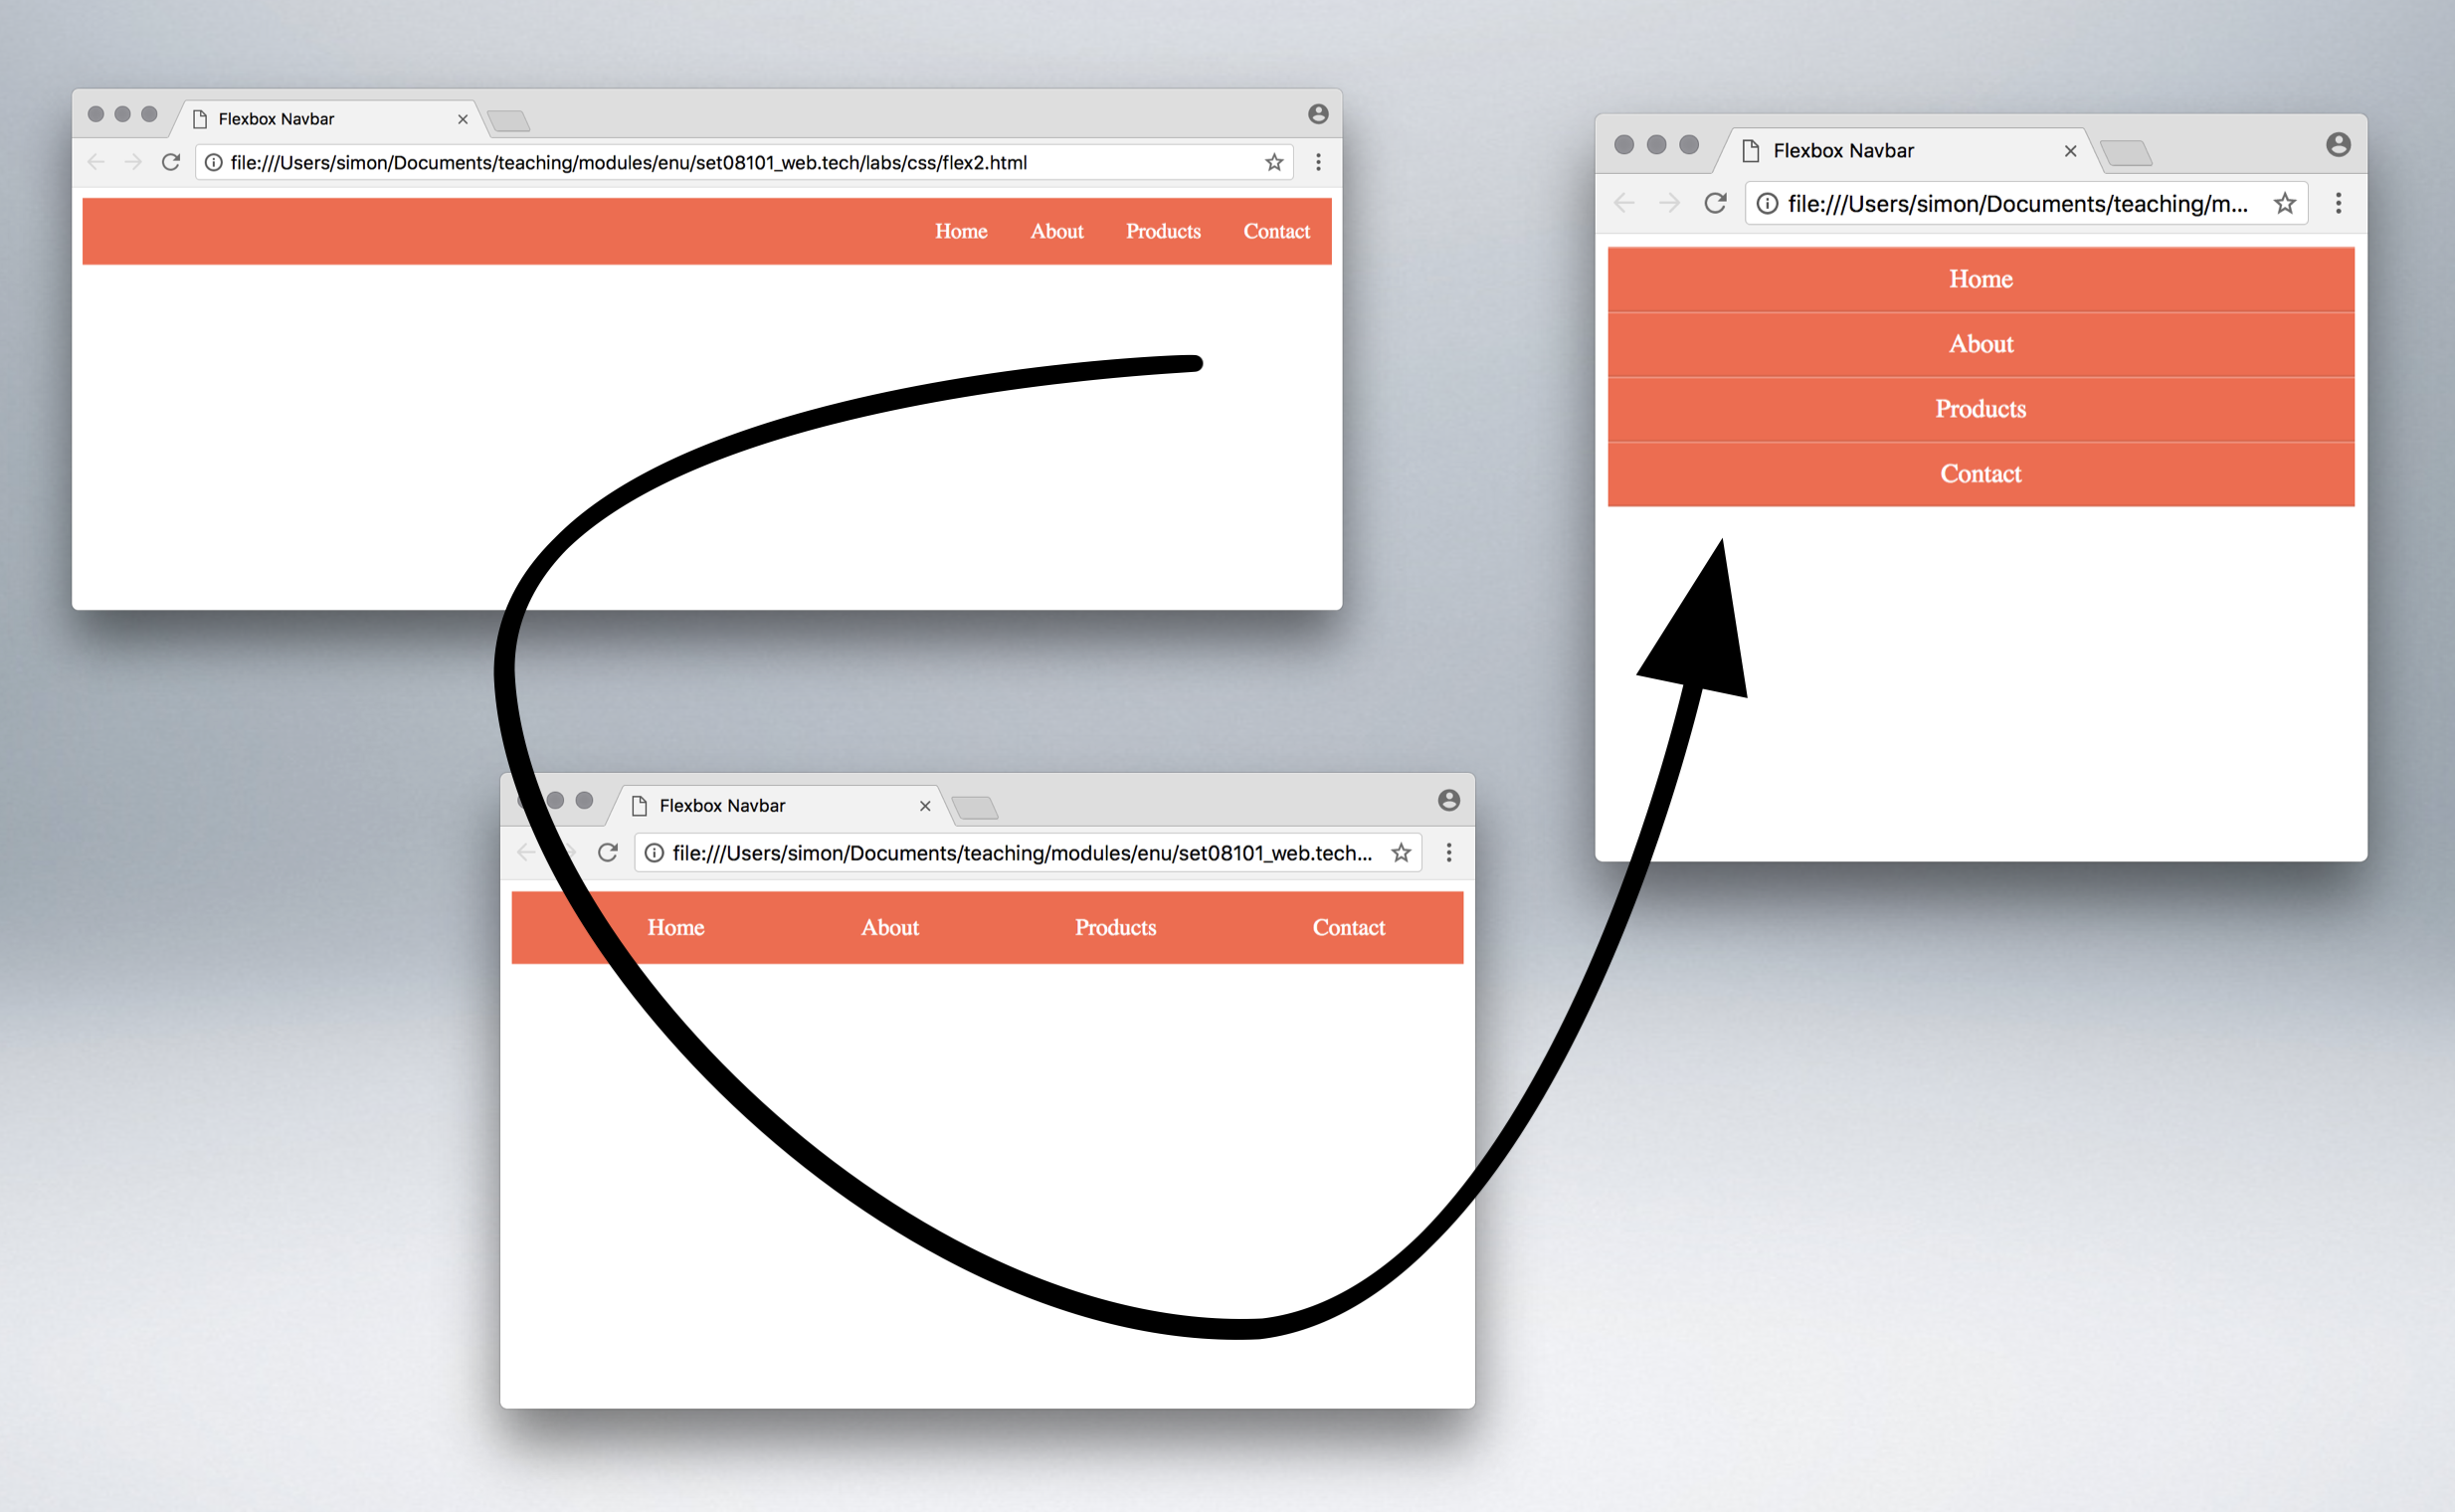
\includegraphics[width=0.8\textwidth]{figures/flexbox-navbar-example}
\label{fig:flexbox-navbar-example}
\caption{}
\end{figure}



\section{Flexbox Page Layouts}
\paragraph{} There's nothing to stop us going further than merely creating a flexible navigation bar. Instead we could use a flexbox to lay out our entire page. Let's give that a go. Note in the example how we are now using semantic HTML5 elements like the header, article, aside, and footer. Note that we're also wrapping everything in a div so that we can apply the display: flex declaration to all of the page's body content. First the HTML (flex3.html
):

\begin{lstlisting}
<!DOCTYPE html>
<html lang="en">
	<head>
		<meta charset="UTF-8">
  		<title>3-column layout + full-width header and footer</title>
  		<link rel="stylesheet" href="flex3.css">
	</head>
	<body>
		<div class="wrapper">
			<header class="header">Yar Pirate Ipsum</header>
  			<article class="main">
    				<p>Deadlights jack lad schooner scallywag dance the hempen jig carouser broadside cable strike colors. Bring a spring upon her cable holystone blow the man down spanker Shiver me timbers to go on account lookout wherry doubloon chase. Belay yo-ho-ho keelhaul squiffy black spot yardarm spyglass sheet transom heave to.</p>  
  			</article>
  			<aside class="aside aside-1">Aside 1</aside>
  			<aside class="aside aside-2">Aside 2</aside>
  			<footer class="footer">Footer</footer>
		</div>
	</body>
</html>
\end{lstlisting}

\paragraph{} Note that we're using some ``placeholder text'' to fill out the various parts of the interface so that the layout engine in the browser actually has something to lay out. Now let's take a look at the CSS (flex3.css):

\begin{lstlisting}
.wrapper {
  display: flex;  
  flex-flow: row wrap;
  font-weight: bold;
  text-align: center;
}

.wrapper > * {
  padding: 10px;
  flex: 1 100%;
}

.header {
  background: #CC3F0C;
}

.footer {
  background: #9A6D38;
}

.main {
  text-align: left;
  background: #33673B;
}

.aside-1 {
  background: #D8CBC7;
}

.aside-2 {
  background: #D8CBC7;
}

@media all and (min-width: 600px) {
  .aside { flex: 1 0 0; }
}

@media all and (min-width: 800px) {
  .main    { flex: 4 0px; }
  .aside-1 { order: 2; } 
  .main    { order: 3; }
  .aside-2 { order: 4; }
  .footer  { order: 5; }
  .header   {order: 1;}
}

body {
  padding: 2em; 
}
\end{lstlisting}

\paragraph{} Now, let's see how that looks. You should be able to recognise a three column layout with full width headers and footers. We should have a resize-able layout that reflows into a sensible order when the window becomes too narrow to accommodate the horizontal layout of the two asides and the main content.

\begin{figure}[H]
\centering
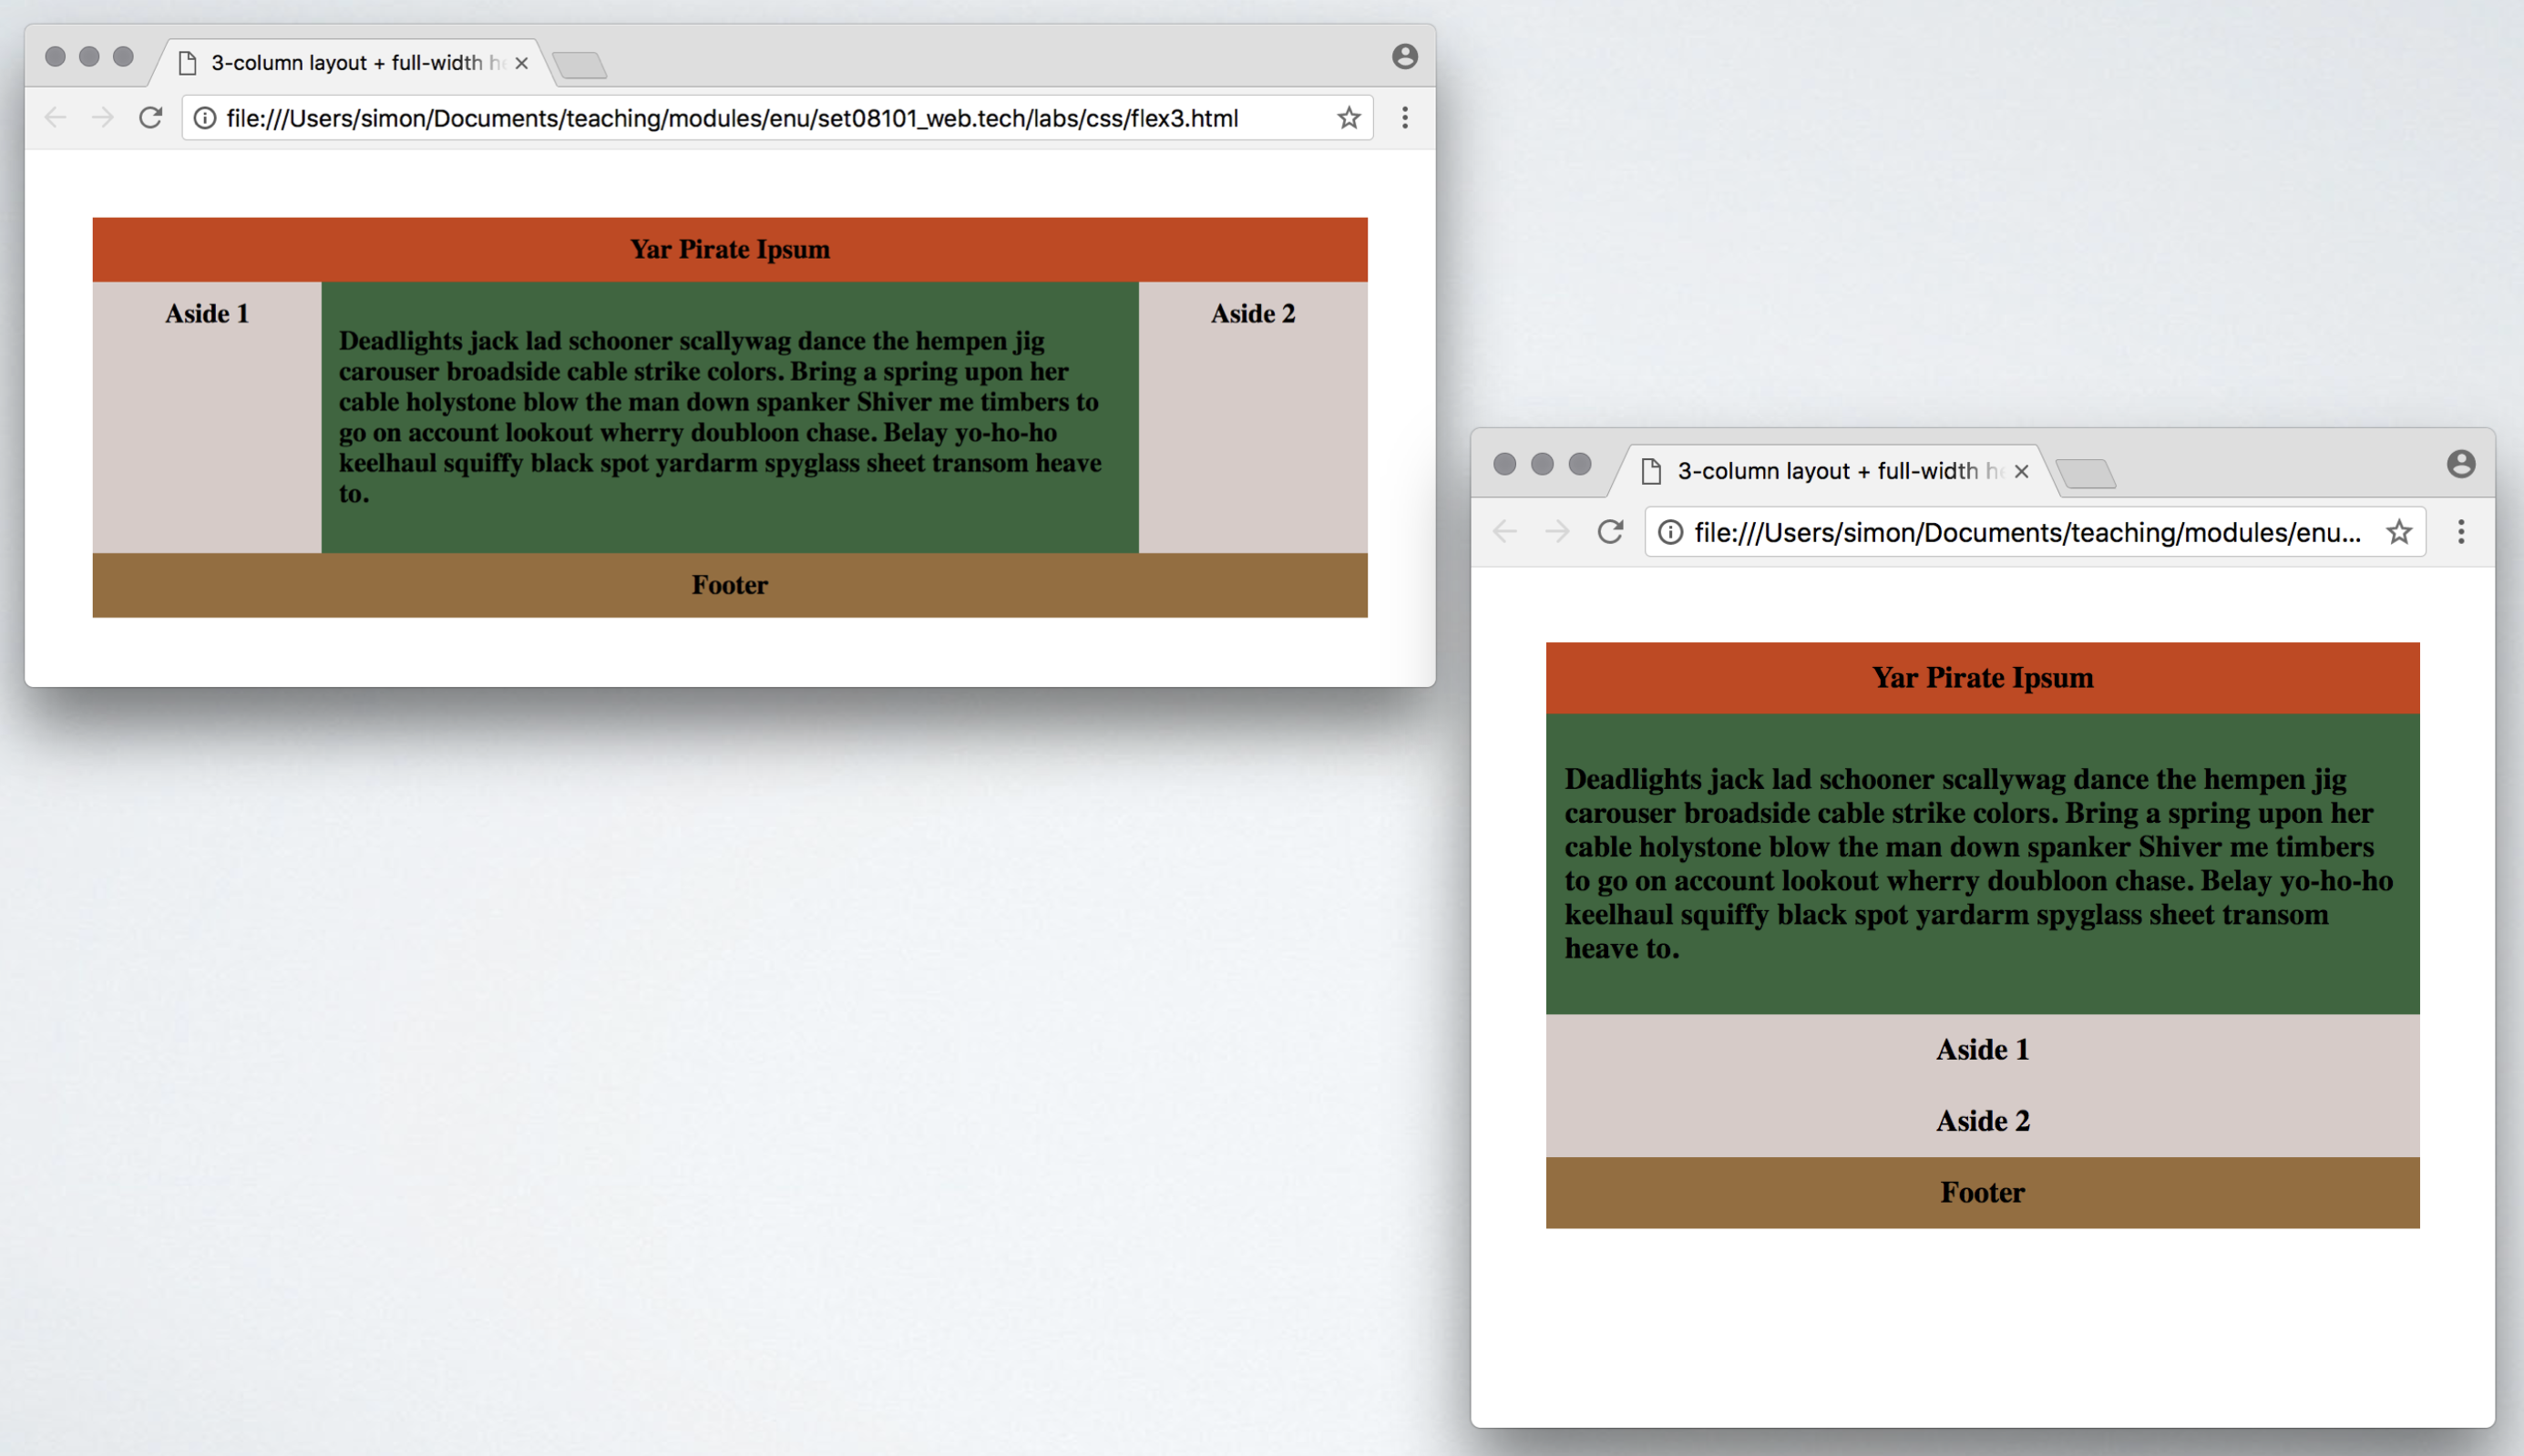
\includegraphics[width=0.8\textwidth]{figures/flexbox-page-layout-example}
\label{fig:flexbox-page-layout-example}
\caption{}
\end{figure}



\section{Flexbox User Interface}
\paragraph{} We can refine this layout easily. With the addition of a slightly nicer colour palette, a little differentiation in text sizes in the various sections, and using the first aside as a navigation panel, we now have something that is a little more visually pleasing. First some HTML (flexbox4.html):

\begin{lstlisting}
<!DOCTYPE html>
<html lang="en">
	<head>
  		<meta charset="UTF-8">
  		<title>Three Column Layout</title>
  		<link rel="stylesheet" href="flexbox4.css">
	</head>
	<body>
  		<header>Header</header>
  		<div class="container">
    			<main>
      				<h1>Main Content</h1>
    			</main>
    			<nav>
      				<h4>Navigation</h4>
    			</nav>
    			<aside>
      				<h4>Aside</h4>
    			</aside>
  		</div>
  		<footer>Footer</footer>
	</body>
</html>
\end{lstlisting}

\paragraph{} Compare this approach to the previous example, again to show you the flexibility of how we can build relatively similar interfaces with different combinations of HTML facilitating the implementation. Note how the header and footer elements are this time outside of the container div that manages the flex layout, i.e., the header and footer are still full width elements at the top and bottom of the screen but are no longer part of the flex layout itself, only the main, nav, and aside elements are part of the FlexBox. Let's take a look at the CSS (flexbox4.css):


\begin{lstlisting}
body {
  margin: 0;
  padding: 0;
  max-width: inherit;
  background: #FFF9F9;
  color: #1C1C1C
}
header{
  font-size: xx-large;
  text-align: center;
  padding: 0.3em 0;
  background-color: #F2EDED;
  color: #1C1C1C;
}
footer {
  font-size: medium;
  text-align: center;
  padding: 0.3em 0;
  background-color: #F2EDED;
  color: #1C1C1C;
}
nav { background: #EDE6E6; }
main { background: #D8DDDE; }
aside { background: #EDE6E6; }
body {
  min-height: 100vh;
  display: flex;
  flex-direction: column;
}
.container {
  display: flex;
  flex: 1;
}
main {
  flex: 1;
  padding: 0 20px;
}
nav {
  flex: 0 0 180px;
  padding: 0 10px;
  order: -1;
}
aside {
  flex: 0 0 130px;
  padding: 0 10px;
}
\end{lstlisting}

\paragraph{} Now let's see how that looks:


\begin{figure}[H]
\centering
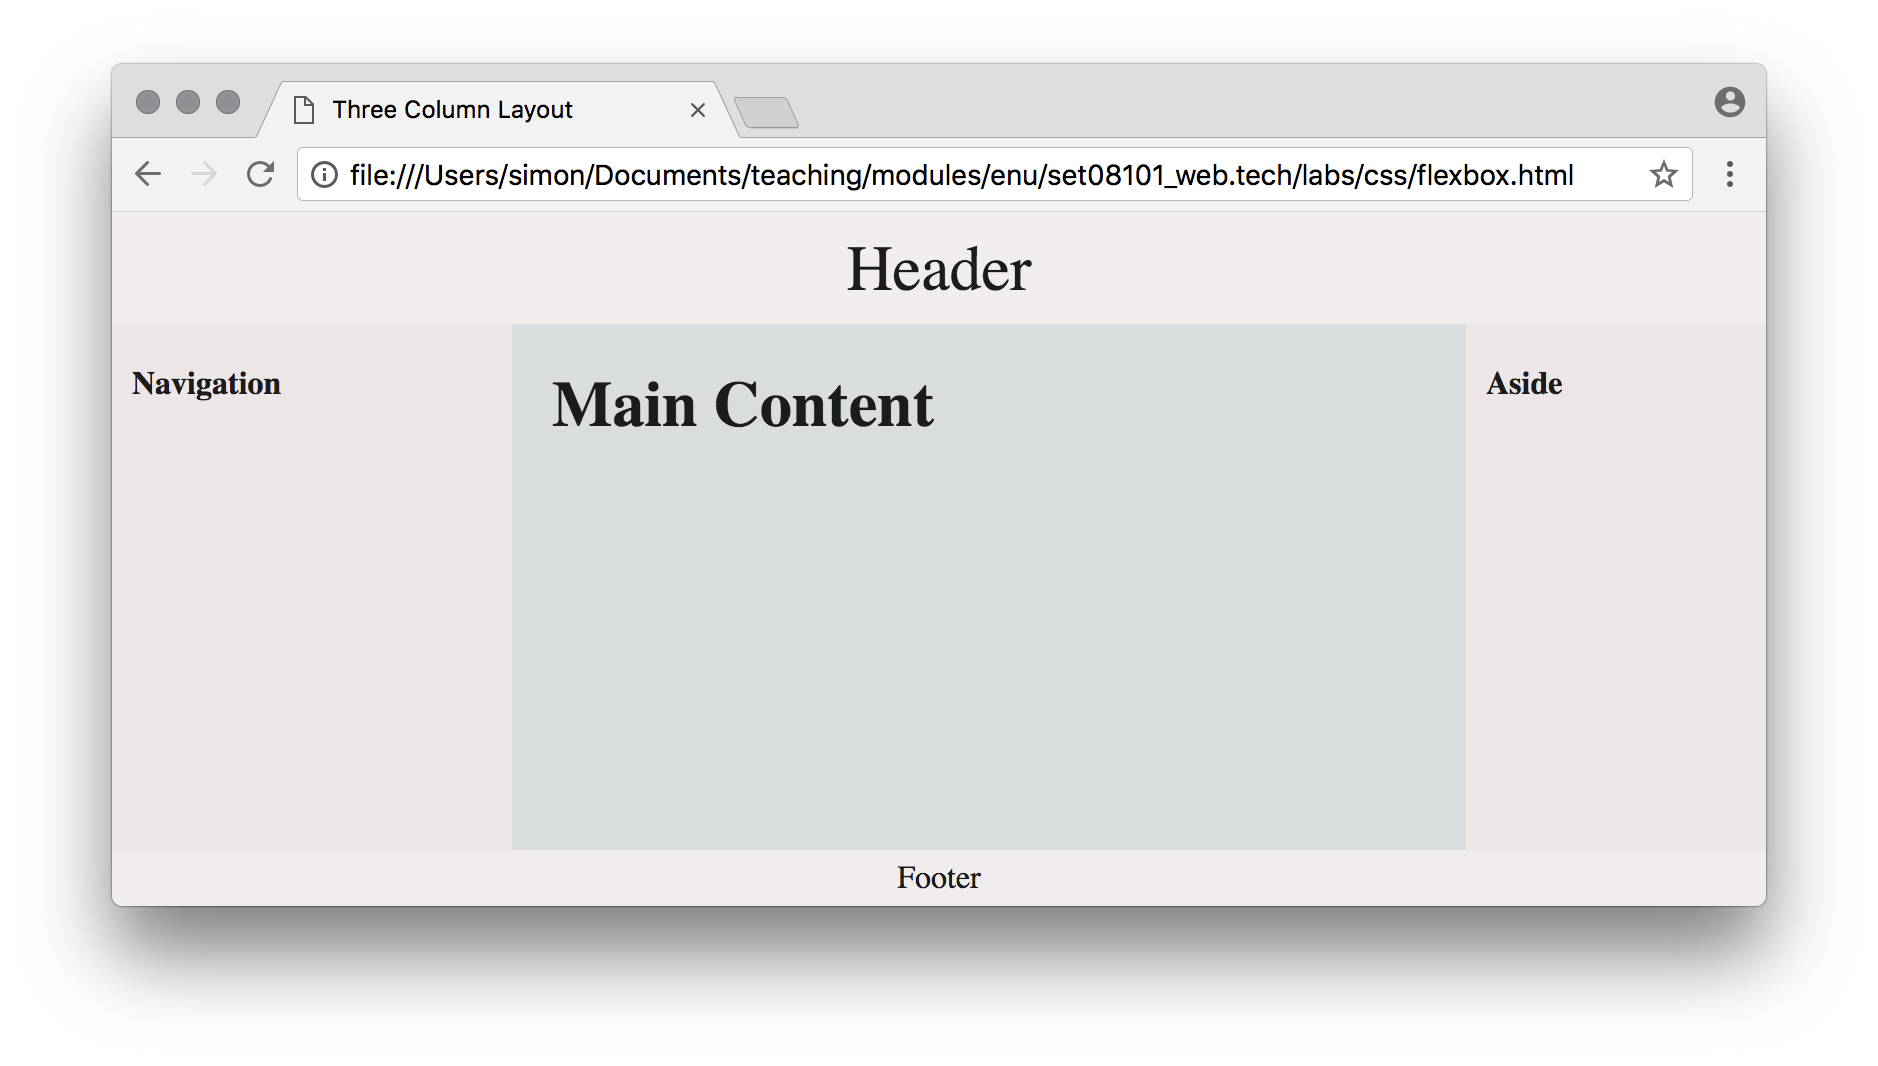
\includegraphics[width=0.8\textwidth]{figures/flexbox-ui-example}
\label{fig:flexbox-ui-example}
\caption{}
\end{figure}



\section{Grid Layout}
\paragraph{} A limitation of the Flexbox is that it works in one dimension. Items in a flexbox are laid out in a line if the page is wide enough and wrapped around as much as needed otherwise. However there is no way to easily force an item to be above or below any other item. That kind of behaviour is within the purview of two-dimensional layout tools, like the Grid layout. Instead of laying out items along a single row, what if we laid out our html elements in rows and columns? Then we could position things above and below each other on screen, independent, to a large degree, of the width of the  bounding window.
\paragraph{} As we mentioned before, this is similar in many ways to the HTML table. However, the HTML table has a semantic meaning, it is concerned only with the organisation of data so that data within the table is related in various ways and organised according to rows and columns.  HTML tables have no visual or presentational meaning in terms of how the resulting table should be displayed, a grid layout is almost the opposite in some ways or rather is a presentational counterpart to the HTML table. On this interpretation, the grid layout has a presentational meaning but the members of the grid have no semantic relation beyond their placement relative to each other, e.g. grid elements in the same row or column aren’t necessarily related and we can't infer any relationship between elements of a grid layout from how it is organised.


\section{Using the Grid Layout}
\paragraph{} We use Grid by setting the display: grid; property on a containing element, e.g. a <div> or even the <body> of the HTML document. This is similar in application to how we used the FlexBox. Essentially it means that we define a containing HTML element to have the grid display property. Then Grid will be used to layout the child elements within that containing element.
\paragraph{} Grid has a number of related properties and values that can be used to control the layout of the grid, e.g. spacing between elements, flow of elements, arrangement of elements.

\paragraph{} The Grid layout supports a range of CSS properties:

\begin{itemize}
\item grid
\item grid-area
\item grid-auto-columns
\item grid-auto-flow
\item grid-auto-rows
\item grid-column
\item grid-column-end
\item grid-column-gap
\item grid-column-start
\item grid-gar
\item grid-row
\item grid-row-end
\item grid-row-gap
\item grid-row-start
\item grid-template
\item grid-template-areas
\item grid-template-columns
\item grid-template-rows
\end{itemize}

\paragraph{} For each property you should investigate the documentation associated with it in the Mozilla developer Network CSS reference\footnote{\url{https://developer.mozilla.org/en-US/docs/Web/CSS/Reference}}. The Grid layout also gives us two basic organisational forms for our layouts, regular or irregular. These are differentiated based upon whether every row and column in the grid has the same number of elements, if they do, then the grid is regular. Otherwise it is irregular. Not all of the layouts that we might want to design will be regular, hence the irregular approach is quite useful when we design web pages. Let's look at examples of each in turn.




\section{Regular Grid Layouts}
\paragraph{} The behaviour of a grid layout is different when resizing a window compared to the same content using the FlexBox property. Compare the behaviour of the following when a window is resized to that of the FlexBox example earlier.


\begin{figure}[H]
\centering
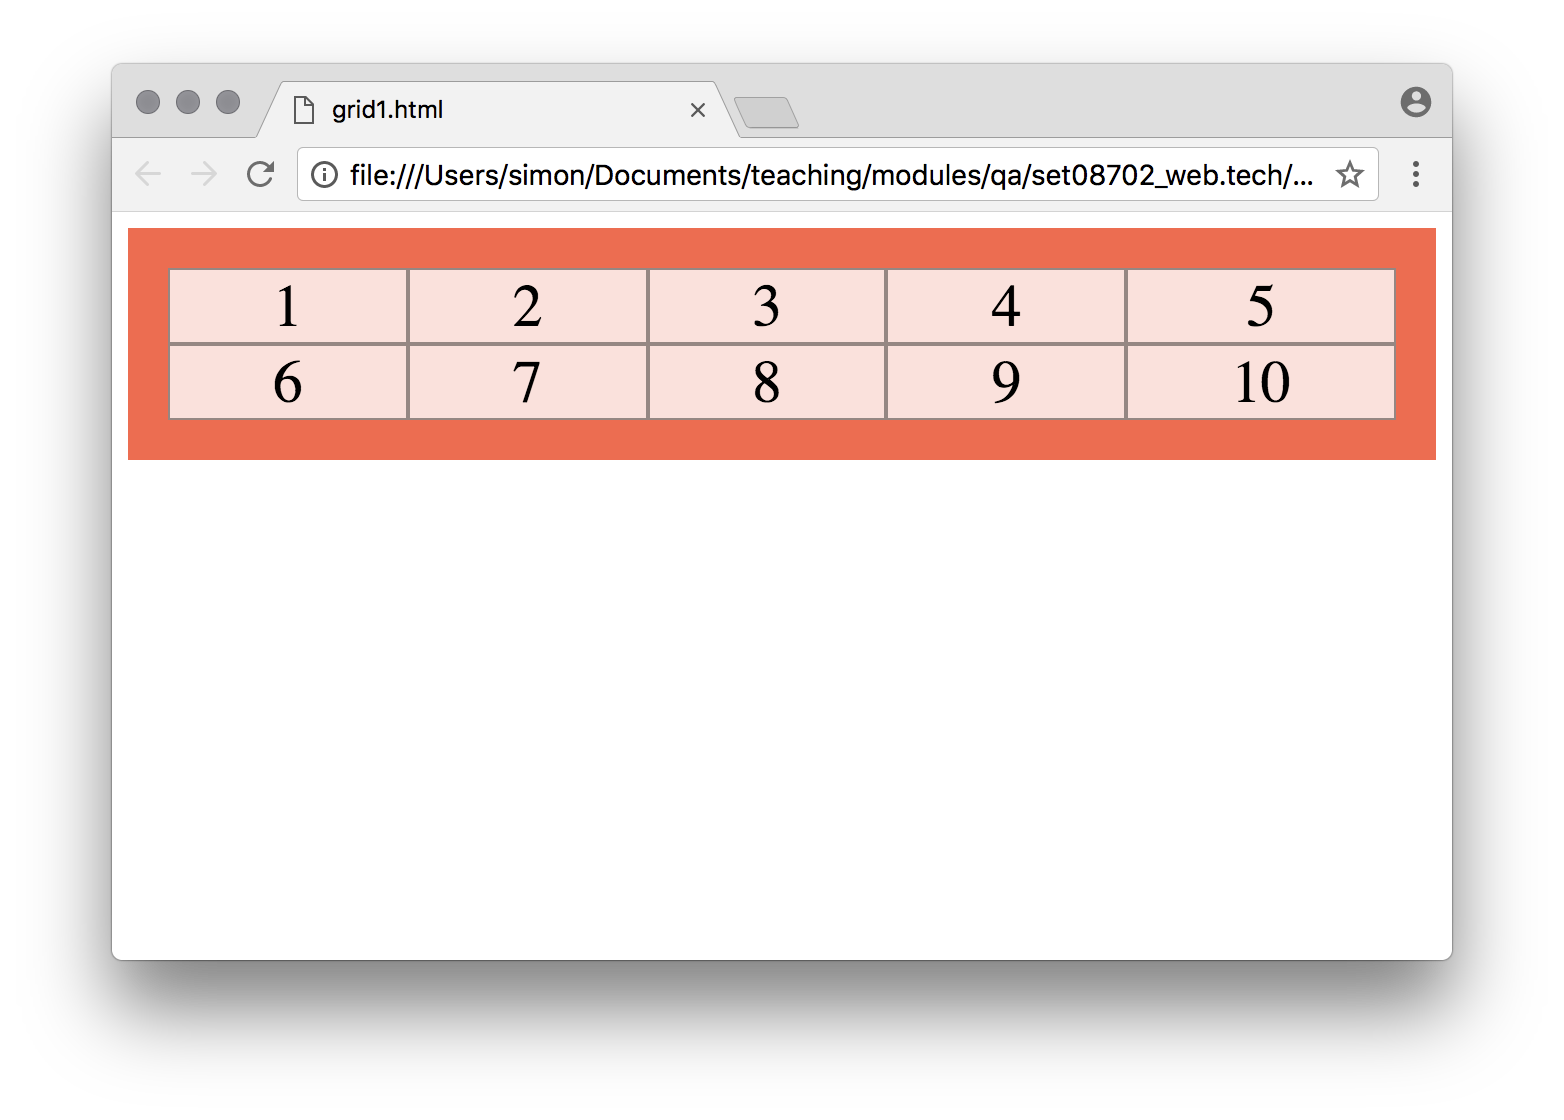
\includegraphics[width=0.8\textwidth]{figures/grid-wide}
\label{fig:grid-wide}
\caption{}
\end{figure}


\paragraph{} Now with a narrower window:

\begin{figure}[H]
\centering
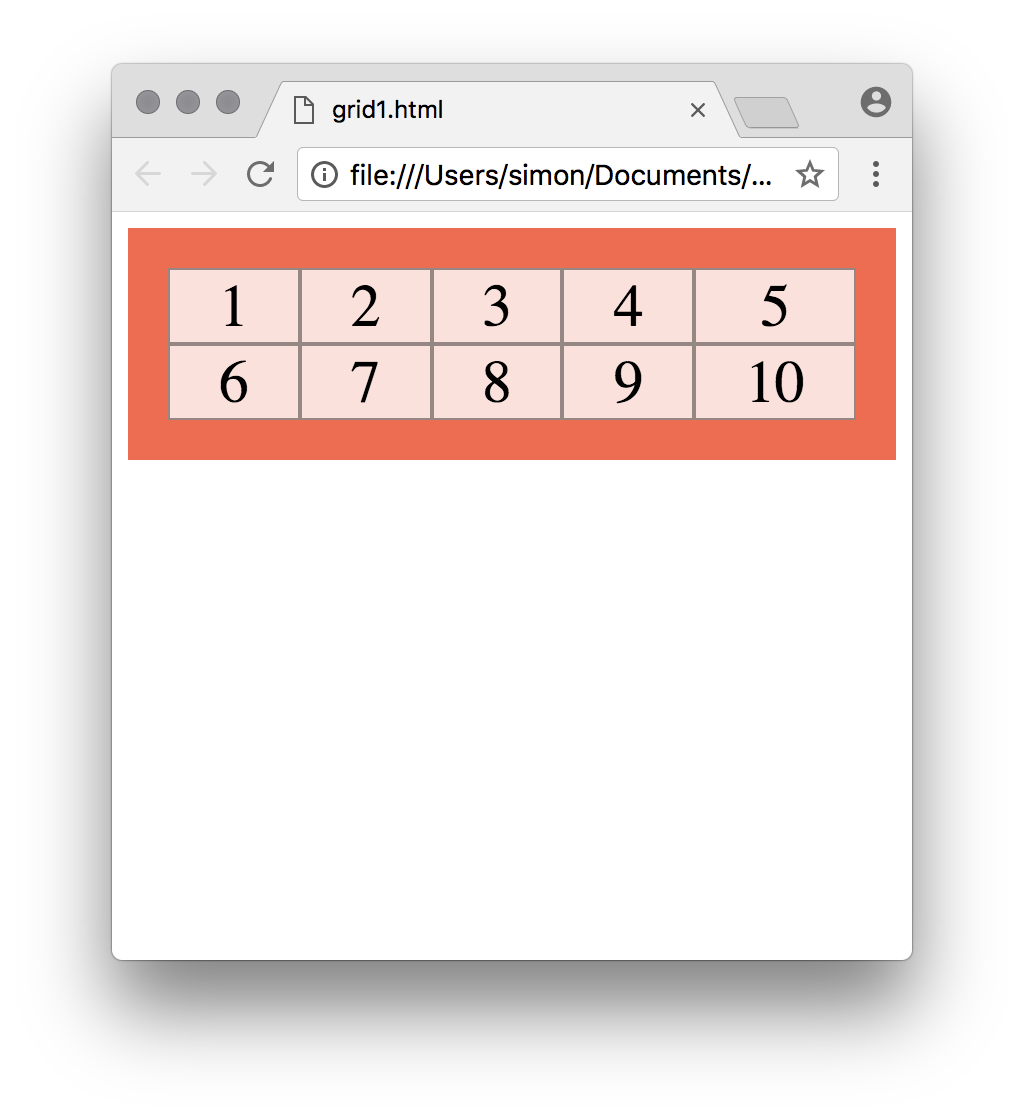
\includegraphics[width=0.8\textwidth]{figures/grid-narrow}
\label{fig:grid-narrow}
\caption{}
\end{figure}


\paragraph{} Notice how it doesn't reflow in the same way. Let's look at how we can implement this in HTML (grid1.html):

\begin{lstlisting}
<!DOCTYPE html>
<html>
	<head>
		<link rel="stylesheet" href="grid1.css">
	</head>
	<body>
		<div class="grid-container">
  			<div class="grid-item">1</div>
  			<div class="grid-item">2</div>
  			<div class="grid-item">3</div>  
  			<div class="grid-item">4</div>
  			<div class="grid-item">5</div>
  			<div class="grid-item">6</div>  
  			<div class="grid-item">7</div>
  			<div class="grid-item">8</div>
  			<div class="grid-item">9</div>
  			<div class="grid-item">10</div> 
		</div>
	</body>
</html>
\end{lstlisting}

\paragraph{} This is a fairly straightforward HTML page whose body contains a div which acts as our container for the items that are meant to be contained by the grid. Each item, in this example, is a piece of text, a number, to differentiate the items from each other. These are then wrapped in div tags and given the grid-item class property so that we can attach some CSS to them. Let's take a look at that CSS(grid1.css):


\begin{lstlisting}
.grid-container {
  display: grid;
  grid-template-columns: auto auto auto auto auto;
  background-color: tomato;
  padding: 20px;
}
.grid-item {
  background-color: rgba(255, 255, 255, 0.8);
  border: 1px solid rgba(0, 0, 0, 0.4);*
  padding: 10px;
  font-size: 30px;
  text-align: center;
}
\end{lstlisting}

\paragraph{} Our CSS is fairly straightforward, some styling for the grid-container, and some styling for the individual grid-items. Note how the container has the display: grid property and we've set the grid-template-columns property to auto so that the browser can determine how big to make the columns based upon the size of the container and the size of the content of each item in the column. We specify the number of columns to create using the auto value in the grid-template-columns property, each declaration of auto specified an additional column, so we end up with five columns in this example.



\section{Irregular Layouts}
\paragraph{} For an irregular layout, which is most useful when designing user interfaces, we can enable individual elements within the Grid to span multiple rows or columns. We achieve this by using the grid-column-start and grid-column-end properties. Let's look at an example that will produce something like the following:


\begin{figure}[H]
\centering
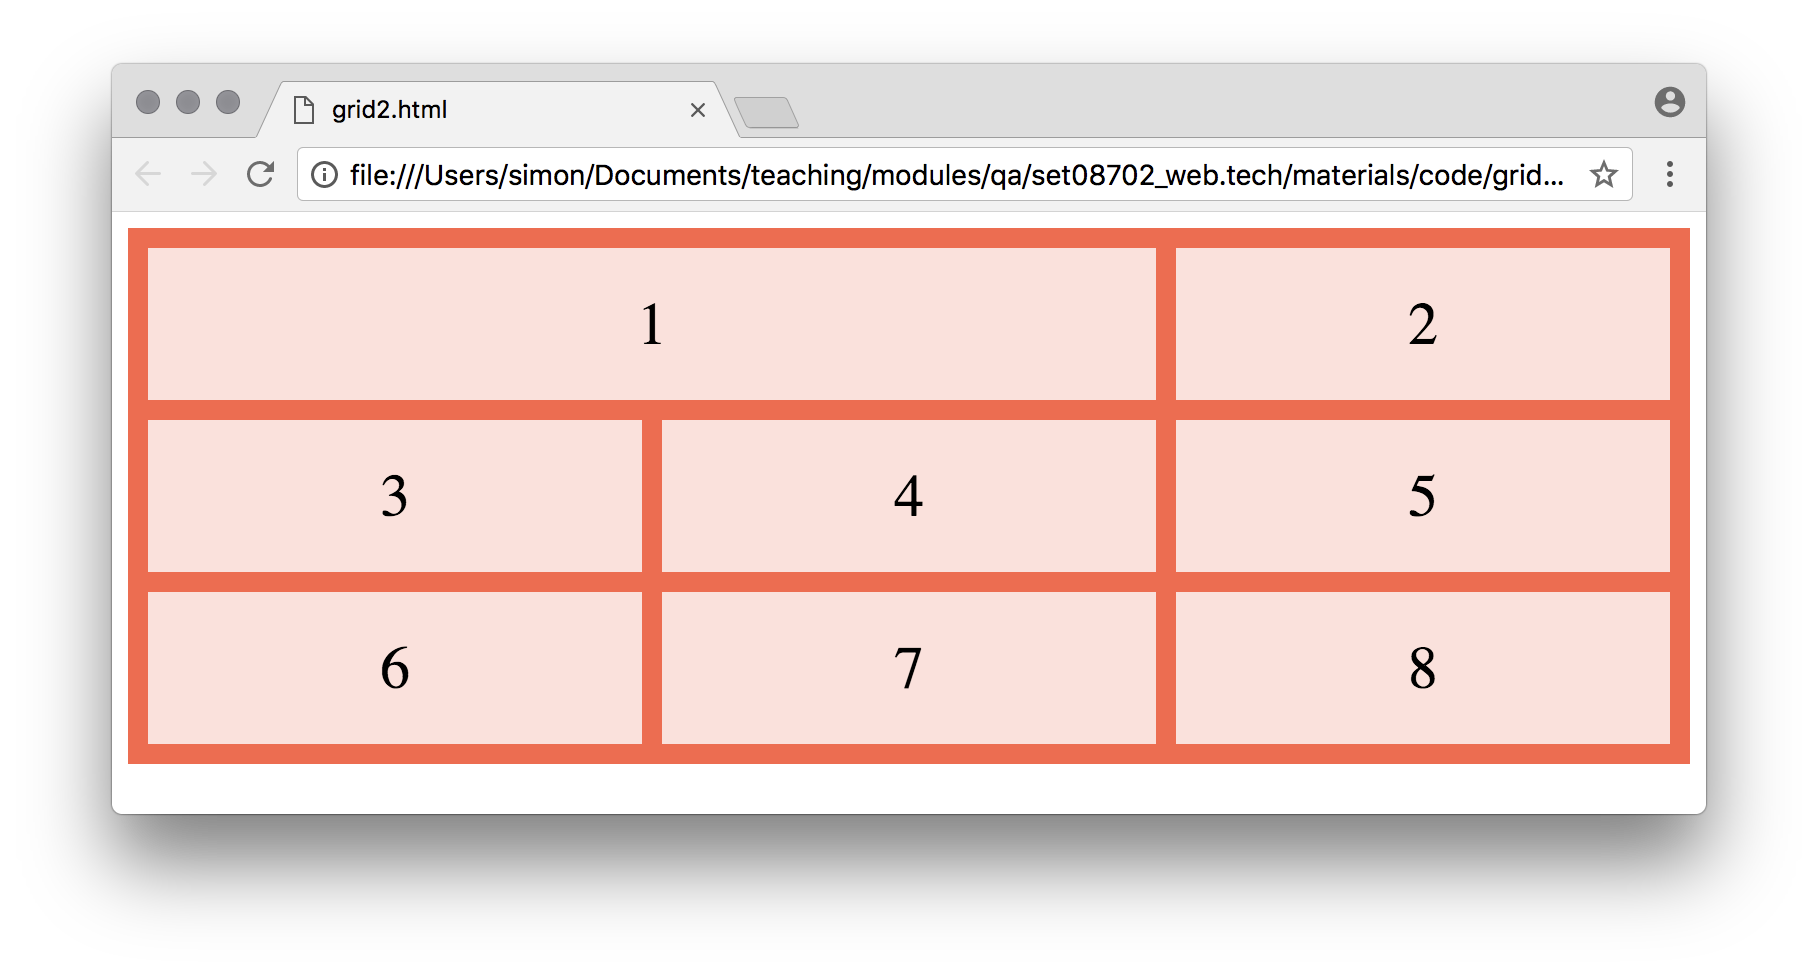
\includegraphics[width=0.8\textwidth]{figures/grid-irregular}
\label{fig:grid-irregular}
\caption{}
\end{figure}


\paragraph{} This can be very useful to give us a pleasing arrangement of the "logical units" that make up the semantic content of our page. First some HTML (grid2.html):

\begin{lstlisting}
<!DOCTYPE html>
<html>
	<head>
		<link rel="stylesheet" href="grid2.css">
	</head>
	<body>
		<div class="grid-container">
  			<div class="item1">1</div>
  			<div class="item2">2</div>
  			<div class="item3">3</div>  
  			<div class="item4">4</div>
 	 		<div class="item5">5</div>
  			<div class="item6">6</div>
  			<div class="item7">7</div>
  			<div class="item8">8</div>  
		</div>
	</body>
</html>
\end{lstlisting}

\paragraph{} Notice that there is very little difference in this HTML compared with that from the regular Grid layout example earlier. The only real differences are that there are two fewer items in this example, and that each item has its own individual class ID. Now the CSS (grid2.css):

\begin{lstlisting}
.grid-container {
  display: grid;
  grid-template-columns: auto auto auto;
  grid-gap: 10px;
  background-color: tomato;
  padding: 10px;
}

.grid-container > div {
  background-color: rgba(255, 255, 255, 0.8);
  text-align: center;
  padding: 20px 0;
  font-size: 30px;
}

.item1 {
  grid-column-start: 1;
  grid-column-end: 3;
}
\end{lstlisting}

\paragraph{} Here we've done almost exactly the same as in the regular layout example but have specified three columns using grid-template-columns: auto auto auto; that is three ``autos'', one for each column. Note that whilst each item has its own individual class ID, we only had to provide individual CSS for  item1 as it is the only one that we wanted to behave differently. Everything else is subsequently laid out using the default Grid layout for a three column grid.



\section{Grid Layout for the User Interface}
\paragraph{} Our examples so far have just looked at how the Grid layout is used. But what about applying it to the design of a user interface layout. This is actually quite similar to our Flexbox Based layout except that it won't reflow in quite the same way as for FlexBox when the window is resized.

\paragraph{} At the expense of reflow flexibility and responsiveness, Grid instead gives us more control over positioning of elements relative to others within the grid. Useful when we want UI elements to appear in specific locations relative to each other.

\paragraph{} A reminder though that the more we try to override the default HTML layout engine in the browser the more effort we must extend to return to the previous responsiveness of raw HTML. Let's take a look at some HTML (grid.html):


\begin{lstlisting}
<!DOCTYPE html>
<html lang="en">
	<head>
  		<meta charset="UTF-8">
  		<title>Modern CSS</title>
  		<link rel="stylesheet" href="grid.css">
	</head>
	<body>
  		<header>This is the header.</header>
  		<main>
    			<h1>This is the main content.</h1>
    			<p>Abluo probo dolore vulpes. Et multo nullus magna inhibeo ex ex quidne conventio sudo pneum. Hendrerit duis vicis at qui iaceo iaceo ut consectetuer reprobo meus.Tincidunt nulla eros erat aliquip laoreet ingenium wisi valde eum. Uxor vel qui validus comis aliquam nutus facilisi feugiat pala.</p>
		</main>
  		<nav>
    			<h4>This is the navigation section.</h4>
    			<p>Pala consequat defui decet at accumsan adipiscing facilisis quis nibh.</p>
  		</nav>
  		<aside>
    			<h4>This is an aside section.</h4>
    			<p>Singularis ullamcorper nimis validus enim genitus demoveo voco et causa. Incassum incassum appellatio pagus augue vindico at in. Quis qui distineo. In abigo consectetuer. Esse populus virtus nisl tum ut nulla ideo vel qui.</p>
  		</aside>
  		<footer>This is the footer.</footer>
	</body>
</html>
\end{lstlisting}


\paragraph{} This should now be looking fairly familiar. An HTML document using some of the HTML5 semantic elements to define the different parts of our interface that we want to lay out. This layout is going to be very similar to our FlexBox layout UI example from earlier. A three column layout with fixed, full-width header and footer. The main difference is the control of the layout using Grid instead of FlexBox and hence different reflow behaviour on window resizing events. The associated CSS (grid.css):

\begin{lstlisting}
body {
  margin: 0;
  padding: 0;
  max-width: inherit;
  background: #fff;
  color: #4a4a4a;
}
header, footer {
  font-size: large;
  text-align: center;
  padding: 0.3em 0;
  background-color: #4a4a4a;
  color: #f9f9f9;
}
nav {  background: #eee; }
main {  background: #f9f9f9; }
aside {  background: #eee; }
body {
  display: grid;
  min-height: 100vh;
  grid-template-columns: 200px 1fr 150px;
  grid-template-rows: min-content 1fr min-content;
}
header {
  grid-row: 1;
  grid-column: 1 / 4;
}
nav {
  grid-row: 2;
  grid-column: 1 / 2;
  padding: 0 10px;
}
main {
  grid-row: 2;
  grid-column: 2 / 3;
  padding: 0 20px;
}
aside {
  grid-row: 2;
  grid-column: 3 / 4;
  padding: 0 10px;
}
footer {
  grid-row: 3;
  grid-column: 1 / 4;
}
\end{lstlisting}

\paragraph{} Which should yield something like the following: A good basic structure for implementing a flexible three column page layout.

\begin{figure}[H]
\centering
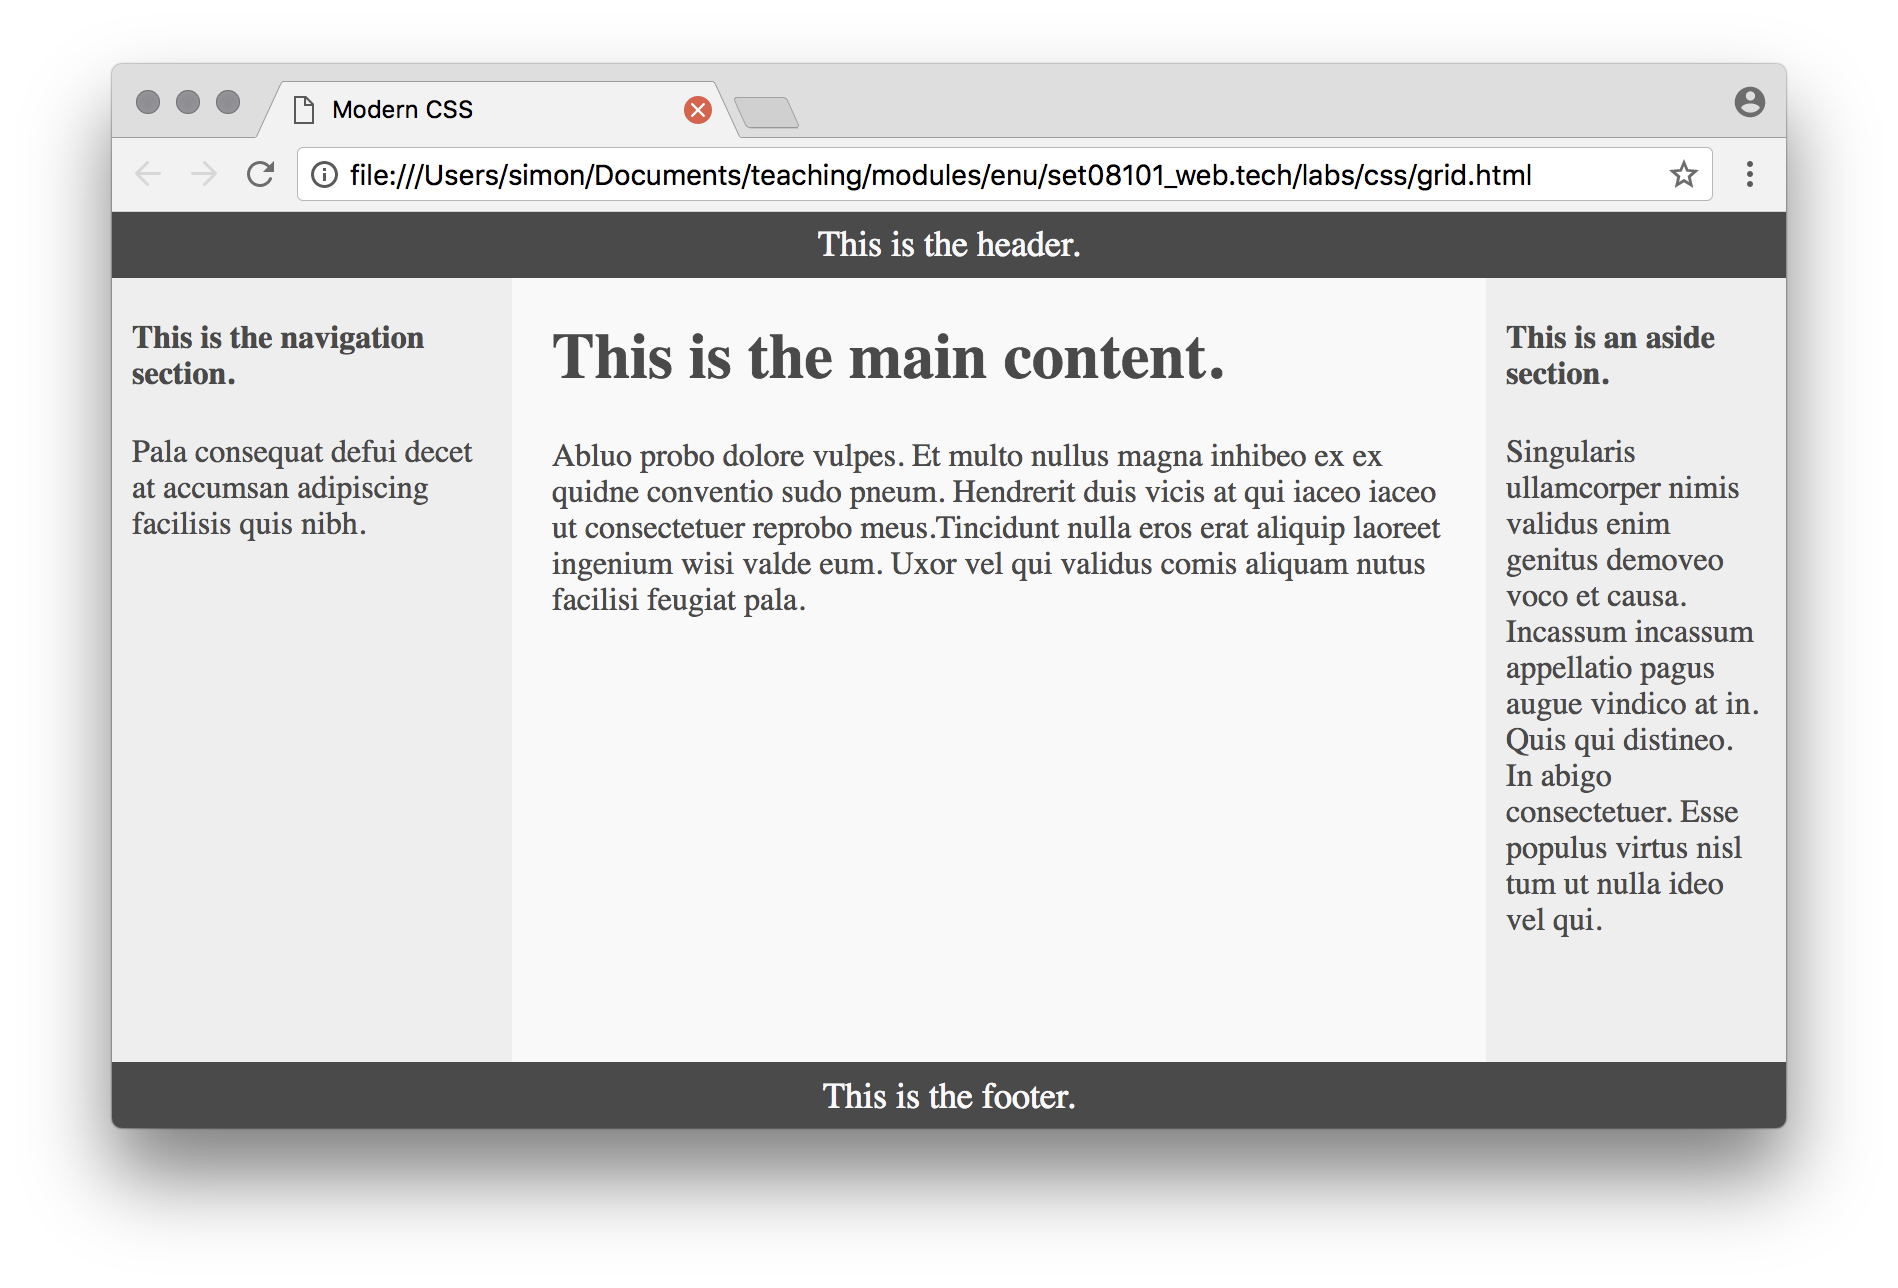
\includegraphics[width=0.8\textwidth]{figures/grid-ui}
\label{fig:grid-ui}
\caption{}
\end{figure}


\section{Summary}
\paragraph{} We should all now have some idea of the various approaches that we can take to place HTML elements within a page. However, under some circumstances, we may want more control over the specific layout of our page and some control over the relative layout of semantic groupings of elements on our page. We can use the Grid and FlexBox layouts to enable this control.

\paragraph{} Beware that beyond this point, increasingly trying to attain pixel perfection in your layout is a road to hurt. This is especially so if you want things to look and act similarly in different browsers which use slightly different layout engines, and the worst case is if you also want similar behaviour in older browsers which can lead to lots of CSS hacks. To my mind CSS hacks, although clever, often feel like a code smell. When we notice them we should perhaps relax and let the browser do more of the work instead of wrestling with it.

